% REV00 Tue 20 Jul 2021 08:12:01 WIB
% START Tue 20 Jul 2021 08:12:01 WIB

\chapter{Limabelas}

% 11
\begin{figure}[htbp]
% h: here, where the figure appears in the text (use can always just use [h] )
% t: top,  top of the current page.
% b: bottom of the current page.
% p: page, top of the next available float space (sometimes end up being the end of the document).
\centerline{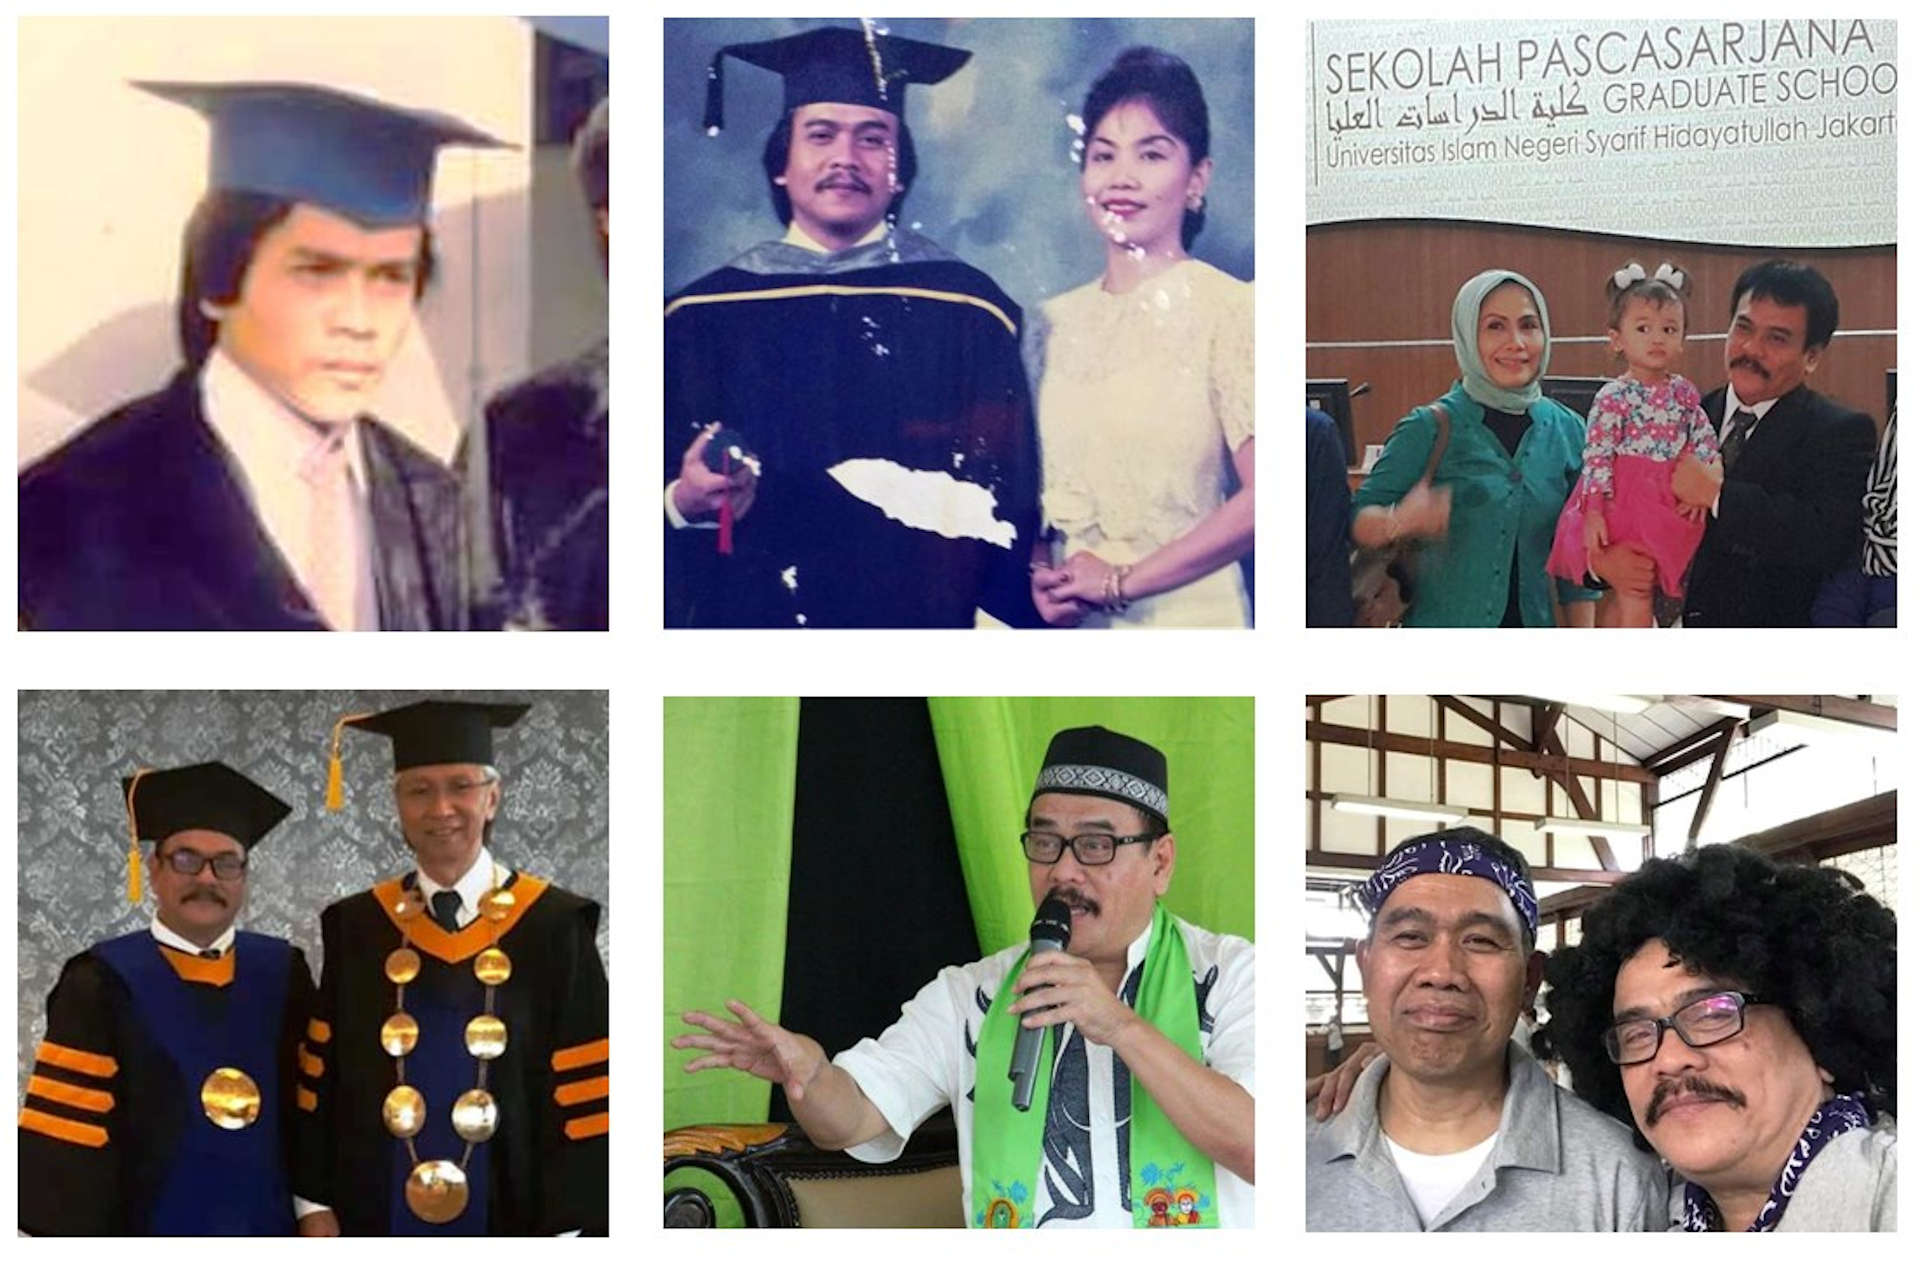
\includegraphics[scale=1.0]{01-15-01}}
\caption{"Galeria (Kika): Wisuda S1, S2, dan S3; Satiri sebagai dosen, sebagai ustadz, dan sebagai sahabat saya" Sumber: Koleksi Marie, FB Satiri, dan Fitria.}
\label{01-15-01}
\end{figure}
%

Mbak Karen, sobatnya, sebelum jadi boss perusahaan minyak negara, ikut membantu Satiri mendirikan perusahaan bersama beberapa teman lainnya: Usaha moving box dan telko yang masih di sekitar perminyakan.

Kebetulan, saya pernah diminta membantu perusahaan ini membenahi dokumen HSE mereka untuk memenuhi syarat prakulaifikasi dalam merebut kontrak di Vico, dlsb.

Dia hanya bisa bertahan tiga tahun di situ. Ada banyak intrik dan tipu daya. Dia terpental. Kekalahan besar, yang harus ia relakan sebagai ongkos belajar.

“Tidak usah marah. Biar Tuhan saja yang membalasnya,” ujarnya kepada Istrinya.

Dengan semua pahit-manisnya itu, kemudian dia bangkit. Membuat dua perusahaan sendiri di bidang IT Solution Provider. Semua dikerjakan sendiri, dan dibantu adiknya, Dian, yang memang menyukai pemrograman.

Tiga tahun berjibaku cukuplah baginya untuk membenturkan kepala: bahwa order harus didapat dengan kongkalikong, sesuatu yang dia makin tidak suka.

“Klien itu enggak mau dikasih produk bagus, Ren. Maunya murah, tapi side-kicknya besar..”

Apalagi sekarang?

Pada dasanya Satiri itu orang jujur. Dia banting setir ke arah yang yang tidak terduga-duga, jauh berbeda. Sisi yang sejak awal kukatakan kepadanya adalah misi yang harusnya dia emban.

Dia teringat pengabdian yang tulus dan cerdas dari guru-gurunya. Dan binar-binar kebahagiaan di mata mereka kala mendapati muridnya yang berhasil.

“Sekarang gua jadi dosen, Ren,” katanya mebuka percakapan setelah beberapa tahun tak berjumpa sejak aku membantunya dengan dokumen HSE. Aku terus terang terpukau.

“Begitu yah?”

“Iya Ren, di universitas kecil di Kebayoran Lama”.

Obrolan itu terjadi sekitar tahun 2008. Aku teringat percakapan dengannya menjelang dia lulus dari ITB awal tahun 1986. Ketika dia ditawari jadi dosen UB, yang kemudian dia tolak untuk jatuh ke pangkuan Schlumberger.

“Abang ingat kan dulu sebelum abang lulus aku bilang bahwa abang itu sangat berbakat jadi dosen? Mungkin memang sekarang waktunya yah…”

“Iya begitu dah…”

“Bang, universitas besar kan banyak. Mengapa ngajar di situ?”

“Nyari duit beneran juga enggak sih…” katanya pelan. Dia bercerita bahwa dia hanya dibayar seharga sebungkus nasi Padang per jamnya. OMG.

“Ren, mahasiswa di situ kebanyakan anak Betawi. Kalau gua enggak ikut ngajar ya siapa lagi?”

Pandangan matanya nanar jauh di belakang punggungku. Mungkin dia sedang melihat binar-binar di mata Bang Ipul dan Pak Paijo!

Di Kebayoran Lama memang masih banyak orang Betawi, dan Universitas itu kecil nyempil persis di sebelahnya Gandaria City: sebuah kompleks mall, hotel dan apartemen yang megah. Lagi-lagi kudapati kontras yang mencolok mata–setelah dulu baby benz boxernya diparkir di sebelah mobil dinas sederhana yang ditumpangi dirjen di kantorku yang lama.

Satiri sedang dalam proses transformasi besar! Usia Satiri saat itu sudah mendekati 50. Anda berani melakukan perubahan besar begitu pada usia seperti itu?

Benarlah, dia memang sedang tidak tertarik untuk mencari uang. Sebagai cadangan dana, selain dana pensiun yang mulai menipis, dia juga membuat beberapa usaha jasa cuci dan setrika pakaian yang sudah berjalan rada mapan.

Di universitas kecil di Kebayoran Lama itu dia belajar jadi dosen. Dan dia belajar dengan cepat.

Berceritalah dia bahwa dia diminta mengajar Matematika Dasar. Di sini, para mahasiswa yang sebagian besar sudah bekerja itu sungguh sangat mencengangkan. Bahkan masih ada yang memahami bahwa 2/3 + 3/4 = 5/7. Ealaah…

Jadi, daripada mengejar target kurikulum, dia lebih memilih untuk mengajar prinsip-prinsip dasar matematika. Persamaan diferensial juga hanya disinggung sedikit sebagai persoalan untuk mengetahui besarnya perubahan, laju atau kecepatan. Integral, hanyalah disinggung bahwa itu adalah alat untuk menghitung nilai keseluruhan, luas atau volume.

Contoh di papan tulis diambil yang paling simpel. Untuk yang rumit, ia menjelaskan cara menggunakan kalkulator internet, seperti integrals.com

Naaah….

Lebih dari itu, dia berupaya mengajarkan perilaku yang baik saja.

Anda tahu bahwa kompetensi seseorang memang dinilai dari pengetahuan, keahlian dan perilakunya. Buat apa pengetahuan dan keahlian yang luar biasa jika perilakunya buruk? Sebaliknya, bukti-bukti di lapangan menunjukkan bahwa karier seseorang akan melaju dengan baik jika perilakunya sangat bagus walaupun didukung dengan pengetahuan dan keahlian yang biasa-biasa saja.

“Kalau anda datang di setiap kuliah saya,” katanya, “Saya akan kasih lulus, berapapun nilai ujianmu nanti!” Naah…

“Koq bisa?”

“Ya kita bikin hiburan deh di setiap pertemuan. Kasih contoh-contoh sederhana penerapan di kehidupan nyata. Gua jamin mereka enggak akan ngantuk…” Itulah kalau orang panggung dan punya pengalaman kerja terus jadi pengajar. Klop!

Bukan hanya memindahkan isi buku ke kepala mahasiswa.

Dia juga berdisiplin dengan waktu. Sekitar satu jam sebelum kuliah dia sudah sampai di kampus. Dia hanya ingin memberikan contoh.

Waktunya banyak sekarang. Lalu apa lagi yang akan ia kerjakan?

Karena banyak di rumah, hobby lama bermain musik jadi tersalurkan bersama istri dan anak-anaknya. Bahkan berkembang ke arah profesional. Pada sekitar tahun dua ribu belasan ini, dia bahkan melayani jasa organ tunggal bersama istri dan anaknya Reza Omo Satiri, yang belakangan sukses dengan grup band-nya sendiri.

Lagu-lagu yang dibawakan macam-macam, bisa dangdut, pop dalam maupun luar negeri, apa saja yang diminta pemilik acara dan penonton. Sebagai biduan utama, Fitria pun tidak pernah canggung membawakannya.

Semakin ia masuk ke industri hiburan ini, semakin ia bergaul dengan lebih banyak orang. Semakin membuatnya melihat dirinya ke dalam: Tetap ada yang terasa kurang!

Bang Maing, adiknya, pernah menceritakan kepadaku bahwa Bang Tiri sempat ‘hilang’ tiga bulan penuh pada periode itu. Ia duduk menekuni 15 jilid Tafsir Al-Mishbah, karangan Prof Shihab. Teman, itu buku tebalnya total tidak kurang dari 75 cm.

Dia menenggelamkan dirinya sebagaimana dulu dia belajar fisika ketika mau ujian.

Satiri tetap mengajar di universitas kecil itu hingga sembilan tahun. Pada masa pengabdiannya itu, dia mengajakku untuk kuliah lagi, kuliah S3. Karena kita sama-sama masih S2.

“Di mana dan belajar apa?” tanyaku.

“Di UIN Ciputat, jurusan Ekonomi Syariah.” Alasannya, kampus itu dekat dengan rumah kami berdua, dan akreditasinya juga baik. Saya memang tinggal di Ciputat dan dia sekarang di Pamulang.

“Kalau kita kuliah bersama kan ada semangat tambahan,” dia mencari teman.

“Lagi pula Ekonomi Syariah itu sedang bangkit..” tambahnya. Tentu saja hal ini tidak bisa saya tolak.

Saya terpukau cukup lama, dan sungguh-sungguh memikirkannya. Namun, dalam hal begini saya cenderung konservatif, mempertahankan prinsip bahwa regulator, pekerjaan saya, tidak membutuhkan S3. Anda tahulah bahwa sekolah super tinggi seperti itu hanya dibutuhkan oleh lembaga penelitian dan universitas.

Saat itu saya segera sadar: Satiri sudah membuat keputusan mengenai akhir kariernya. Sebagai pendidik!

“Okay, aku pikirkan dulu dana dan waktunya ya Bang…” Dia tahu aku hanya berbasa-basi.

.
***

Kepiawaian Satiri kecil mengaji dan kemampuan abstraksi fisikanya membuat ia mudah untuk memahami kitab suci di tingatan hakikat, bukan sekedar persyaratan hukum formal semata.

Buat saya itu adalah state of the art, the end-state of a genius journey.

Penguasaan panggung, vokal yang bagus, dan akhirnya dia memilih bahasa yang sangat sederhana yang mudah dipahami siapa saja, serta dengan kutipan Kitab yang sesekali saja.

“Orang pastinya menginginkan ajaran yang bagus, ilmiah dan bermakna,” katanya suatu ketika seusai memberikan Khutbah Jumat di kantorku. Aku hanya bisa menatap dinding di belakang punggungnya. Mengingat kembali seorang Buya yang dihormati orang setanah air. Ketika agama memberikan kedamaian bagi semesta.

Dengan kemampuan itu, pada pertengahan 2015 lalu ia menyelesaikan S3 di UIN hanya dalam dua tahun saja. Dan seperti biasa, hasilnya cum laude.

Sebagian orang kini memanggilnya ustadz, sebagian Pak Dosen. Kepada teman-teman kuliah atau sobat gaul, ia lebih suka dipanggil Bang Tiri, dan bahkan BangSat.

Untuk membuktikan keseriusan ilmu yang didapatnya, mulai 2016 dia menjadi ketua program Intenational Business Administration di universitas swasta pemula yang cukup bergengsi, International University Liaison Indonesia di kawasan Serpong. Sekolah garapan Ilham Habibie yang bekerjasama dengan universitas di Jerman.

Saya tahu dia adalah tipe dosen yang disukai mahasiswa. Ganteng, pintar, humoris, namun memilih bahasa dan penampilan yang sederhana. Pasti di sini ada muridnya ikut membaca. Naah…

Satiri juga terus menjadi ustadz. Di kompleks rumah saya pernah kami undang sebagai pemberi khotbah di hari raya. Semua menyukainya, bahkan Panitia menyebutnya sebagai Prof. Ya, dia diundang dimana-mana.

Tanpa tarif, karena bukan itu juga yang ia harapkan. Walaupun dia tidak lagi memiliki harta sebanyak ia mau menangguknya di sungai penuh minyak. Itu dahulu. Tetapi sekarang wajahnya jauh lebih cerah.

Dia bahagia.

Apakah menjadi dosen dan ustadz membuatnya membatasi diri atau kurang gaul?

Salah, ia malah aktif dimana-mana. Dia tetap ada di ORARI maupun RAPI, Bamus Betawi, Gerbang Betawi, Betawi Rawa Belong, Ikatan Penyanyi Musisi Indonesia (IPMI) Tangsel, dan bahkan di YNCI Tangsel, solidaritas pengendara sepeda motor. Sebagian ia ikut jadi pengurus, sebagian sebagai pembina.

Dia ingin lebih banyak mengajarkan disiplin, mengajarkan cara berpikir yang benar, dan semuanya melalui contoh prestasi dan budi baik saja. Bukan lagi dengan kata-kata. Dan dia memilih semesta yang ia berpihak untuk mereka: Orang-orang di bawah, dan yang hampir menengah.

Dia punya ruang belajar lebih besar, bukan sekedar ruang kelas atau rumah ibadah.

Tiga Jum’at yang lalu, pada tanggal 25 Juni 2021 Tuhan memanggilnya. Dan ia sudah berdamai dengan semua yang dialaminya, dan semua yang disayanginya. Dia tetap menyandang predikat pengajar terbaik di universitasnya!

EPILOG

Di malam saya mendengar khabar kepergiannya, saya tidak malu-malu menangis di sebelah istri saya. Bercucuran air mata. Setelah puas, saya segera mengambil laptop. Menulis tentangnya selama dua malam berurut-turut hingga subuh.

Dia telah menemani dan membuat saya mampu menuliskannya.

Siapapun yang mengenal Satiri saya kira berkewajiban menuliskan biografinya semampu mereka. Dan menyebar-luaskannya. Sebab, Satiri adalah tentang perjuangan, cita-cita, kasih-sayang, keluarga, pendidikan dan kebaikan, serta kegembiraan hidup yang harus dihidupkan.

Mengapa saya menuliskannya segera setelah kepergian beliau?

Karena saya tidak punya PERSEMBAHAN apapun untuk mengiringi kepergiannya selain dengan tulisan ini. Saya tentu tidak bisa menyembahnya. Dan, saya juga tidak mungkin mengirimkan bunga ke rumah atau makamnya.

Sepanjang hidupnya adalah rangkaian bunga yang indah, dan dia sendiri adalah ahlinya. Persembahan kembang dari saya hanya akan menjadi kesia-siaan. Bahkan menjadi sampah dalam tiga hari saja. Dan sangat merepotkan untuk membuangnya.

Mengapa saya bersusah payah menulis tentang Satiri?

Tidak terlalu sulit bagi saya untuk menuliskannya, karena dia adalah pahlawan saya. Di era pandemi ini, kita membutuhkan pahlawan untuk saling menguatkan.

Sekarang, biarkan saya bertanya padamu: Siapa pahlawanmu?

.
Catatan:
Terima kasih atas masukan ibu-bapak dan teman-teman semua yang mengusulkan agar saya menulis biografi lengkap Satiri. Usulan yang sangat mulia. Saya akan memikirkannya dengan sungguh-sungguh. Tahun ini kebetulan ada amanah kerja yang cukup besar yang harus saya garap dengan sabar. So, sabar yaa…

Al Fatihah buat Bang Tiri, dan salam sehat buat kita semua.
\\[10pt]

Sumber tulisan asli \url{https://www.facebook.com/reno.alamsyah.94/posts/10226615176551698}

